\documentclass[10pt,twocolumn]{article}

\usepackage{times}
\usepackage{fullpage}

\usepackage{booktabs}  % for \midrule
%\usepackage{subfigure}
\usepackage{balance}
\usepackage{graphicx}
\usepackage{xspace}
%\usepackage{pslatex}
%\usepackage{pifont}
%\usepackage{multirow}
%\usepackage{array}
%\usepackage{booktabs}
%\usepackage{cite}
\usepackage{url}
%\usepackage{cancel}
\usepackage{color,colortbl}
%\usepackage{microtype}
%\usepackage{textcomp}% http://ctan.org/pkg/textcomp
\usepackage{tabularx}
\usepackage{framed}
\usepackage[]{algorithm2e}
\SetAlFnt{\small}
\SetAlCapFnt{\small}
\usepackage{algorithmic}

\usepackage{listings}
%\usepackage{scrextend}
\usepackage{mathtools}
\usepackage{pbox}

\let\labelindent\relax
\usepackage{enumitem}

\usepackage[labelfont=bf]{caption}

%\theoremstyle{plain}
\newtheorem{theorem}{\bf{Theorem}}%[section]
\newtheorem{lemma}[theorem]{\bf{Lemma}}
\newtheorem{corollary}[theorem]{\bf{Corollary}}
\newtheorem{proofl}[theorem]{\bf{Proof}}
\newtheorem{proposition}[theorem]{\bf{Proposition}}

%\theoremstyle{definition}
\newtheorem{definition}{\bf{Definition}}%[section]
\newtheorem{observation}{\bf{Observation}}%[section] 

%\theoremstyle{remark}
\newtheorem{example}{\bf{Example}}
\newtheorem{notation}{\bf{Notation}}
\newtheorem{fact}{\bf{Fact}}

\usepackage{listings}
\lstdefinelanguage{cs}
{
  morekeywords={abstract,event,new,struct,as,explicit,null,switch
		base,extern,this,bool,false,operator,throw,
		break,finally,out,true,byte,fixed,override,try,
		case,float,params,typeof,catch,for,private,uint,
		char,foreach,protected,ulong,checked,goto,public,unchecked,
		class,if,readonly,unsafe,const,implicit,ref,ushort,
		continue,in,return,using,decimal,int,sbyte,virtual,
		default,interface,sealed,volatile,delegate,internal,short,void,
		do,is,sizeof,while,double,lock,stackalloc,
		else,long,static,enum,namespace,string,
		where, from, select, group,by, having, into, many,
		every,
                function,
		or, and, on, var, when,let, zip, combine,
		minute,hour,day,week,year,calendar,count, Delay, Until, TakeUntil, Sample, Skip, Throttle},
	  sensitive=true,
	  morecomment=[l]{//},
	  morecomment=[s]{/*}{*/},
	  morestring=[b]",
}

\lstset{
	language=cs,
	tabsize=2,
        basicstyle=\small,
%        basicstyle=\normalsize,
        %upquote=true,
%        aboveskip={1.5\baselineskip},
        columns=fullflexible, %fixed,
        showstringspaces=false,
        extendedchars=true,
        breaklines=true,
%      prebreak = \raisebox{0ex}[0ex][0ex]{\ensuremath{\hookleftarrow}},
%	frame=single,
        showtabs=false,
        showspaces=false,
       identifierstyle=\ttfamily,
        keywordstyle=\color[rgb]{0,0,.8},% \sffamily,
        commentstyle=\color[rgb]{0.133,0.445,0.133},
%        stringstyle=\color[rgb]{0.627,0.126,0.941},
	numbers=left,
	xleftmargin=17pt,
%	tabsize=2
	captionpos=b,
	breakatwhitespace=true,     % sets if automatic breaks should only happen at whitespace
}

\newcommand\mypara[1]{\vspace{.3em}\noindent\textbf{#1}}
\newcommand{\urlwofont}[1]{\urlstyle{same}\url{#1}}

\newcommand{\dinv}{Dinv\xspace}
\newcommand{\dviz}{Dviz\xspace}

%%%%%%%%%%%%%%%%%%%%%%%%%%%%%%%%%%%%%%%%
% Useful reviewing/feedback annotations
\usepackage{ifthen}
\usepackage[normalem]{ulem} % for \sout
\usepackage{xcolor}
\usepackage{amssymb}

\newcommand{\ra}{$\rightarrow$}
\newboolean{showedits}
\setboolean{showedits}{true} % toggle to show or hide edits
\ifthenelse{\boolean{showedits}}
{
	\newcommand{\ugh}[1]{\textcolor{red}{\uwave{#1}}} % please rephrase
	\newcommand{\ins}[1]{\textcolor{blue}{\uline{#1}}} % please insert
	\newcommand{\del}[1]{\textcolor{red}{\sout{#1}}} % please delete
	\newcommand{\chg}[2]{\textcolor{red}{\sout{#1}}{\ra}\textcolor{blue}{\uline{#2}}} % please change
}{
	\newcommand{\ugh}[1]{#1} % please rephrase
	\newcommand{\ins}[1]{#1} % please insert
	\newcommand{\del}[1]{} % please delete
	\newcommand{\chg}[2]{#2}
}

\newboolean{showcomments}
%\setboolean{showcomments}{true}
\setboolean{showcomments}{false}
\newcommand{\id}[1]{$-$Id: scgPaper.tex 32478 2010-04-29 09:11:32Z oscar $-$}
\newcommand{\yellowbox}[1]{\fcolorbox{gray}{yellow}{\bfseries\sffamily\scriptsize#1}}
\newcommand{\triangles}[1]{{\sf\small$\blacktriangleright$\textit{#1}$\blacktriangleleft$}}
\ifthenelse{\boolean{showcomments}}
%{\newcommand{\nb}[2]{{\yellowbox{#1}\triangles{#2}}}
{\newcommand{\nbc}[3]{
 {\colorbox{#3}{\bfseries\sffamily\scriptsize\textcolor{white}{#1}}}
 {\textcolor{#3}{\sf\small$\blacktriangleright$\textit{#2}$\blacktriangleleft$}}}
 \newcommand{\version}{\emph{\scriptsize\id}}}
{\newcommand{\nbc}[3]{}
 \renewcommand{\ugh}[1]{#1} % please rephrase
 \renewcommand{\ins}[1]{#1} % please insert
 \renewcommand{\del}[1]{} % please delete
 \renewcommand{\chg}[2]{#2} % please change
 \newcommand{\version}{}}
\newcommand{\nb}[2]{\nbc{#1}{#2}{orange}}

\definecolor{ibcolor}{rgb}{0.4,0.6,0.2}
\newcommand\iv[1]{\nbc{IB}{#1}{ibcolor}}
\usepackage{wasysym}
\newcommand\yesml[1]{\nbc{ML {\textcolor{yellow}\sun}}{#1}{mircolor}}

\definecolor{sgcolor}{rgb}{0.2,0.0,0.5}
\newcommand\sg[1]{\nbc{SG}{#1}{sgcolor}}

\definecolor{samcolor}{rgb}{0.2,0.4,0.2}
\newcommand\sam[1]{\nbc{SC}{#1}{samcolor}}

\definecolor{hccolor}{rgb}{0.21,0.54,0.84}
\newcommand\hc[1]{\nbc{HC}{#1}{hccolor}}

% Todo Command
\definecolor{todocolor}{rgb}{0.9,0.1,0.1}
\newcommand{\todo}[1]{\nbc{TODO}{#1}{todocolor}}


%%%%%%%%%%%%%%%%%%%%%%%%%%%%%%%%%%%%%%%%

\begin{document}

%\title{Inferring likely data invariants of distributed systems}
\title{Visualizing Distributed State}
\author{Zipeng Liu\\
    \textit{zipeng@cs.ubc.ca}
    \and
    Stewart Grant\\
    \textit{sgrant09@cs.ubc.ca}
}
\date{}
\maketitle
\thispagestyle{empty}

\section{Abstract}
\label{sec:abstract}
%%%%%%%%%%%%%%%%%%%%%%%%%%%%%%%%%%%%%%%%%%%%%


Understanding distributed systems is difficult. Concurrency and
non-determinism leads developers to misinterpret their systems
behaviour. Indeed, even small systems require complex reasoning to
determine if their behaviour is correct.  Developers
characteristically log executions; when unspecified or deviant
behaviour is observed, the culprit is determined through laborious log
inspection. Specifications are useful for defining correct behaviour,
but proving that a system adheres to a specification is beyond the
capabilities of modern techniques.  Such shortcomings demand new tools
to help developers better understand their systems, and quickly
identify deviant behaviour.  Using visualizations, large amounts of
information can be concisely, and meaningfully encoded. Distributed
state, communication patterns, and data invariants are useful
execution artifacts for reasoning about a systems behaviour.  However,
interpreting them from logs alone is tricky and error prone.  We
propose Pangaea, a tool for identifying deviant behaviour in
distributed systems.  Using novel distributed state differentiation
Pangaea builds approximate, high level, finite state machines derived
from dynamic behaviour. Deviations from expected state machines can be
inspected using a graph of the systems invariants, and communication
graph. \textbf{We evaluated Pangaea$\dots$}.

%%%%%%%%%%%%%%%%%%%%%%%%%%%%%%%%%%%%%%%%%%%%%
\section{Introduction and Motivation}
\label{sec:intro}
%%%%%%%%%%%%%%%%%%%%%%%%%%%%%%%%%%%%%%%%%%%%%

The behaviour of distributed systems is often complicated and
difficult to understand. Even small simple systems require that
developers reason about concurrency, and the possibility of
communication and node failure. In order to develop correct systems
and triage bugs developers must construct a mental model for how
their system should behave. Typically distributed systems are built by
first strictly specifying the system, then developing the system to the
specification. This approach has the advantage that the specification
can be verified, and that it helps developers build mental models of
their systems prior to writing
code~\cite{Newcombe:2015:AWS:2749359.2699417,WilcoxWPTWEA2015}.
Distributed system specification are simplified versions of the
software which define finite state machines (FSM), and invariants
based on protocol specific behaviour. FSM are much easier to reason
about than source code, and provide developers an intuitive
understanding of how their system should behave in all cases.
Invariants are likewise useful in that they constrain the behaviour of
a system which shrinks the space of behaviours developers need to
reason about. However, specifications are not source code. As
implementations grow they drift further from their abstract
specifications~\cite{917525}. When bugs occur developers typically use
a systems logs to triage the problem. These logs can be massive, and
identifying buggy behaviour is a laborious error prone task.  In order
to understand their real systems developers require tools which can
communicate complicated concurrent behaviour. Tracing tools such as
Dapper~\cite{36356}, and Lprof~\cite{Zhao:2014:LNR:2685048.2685099}
are useful for reasoning about specific behaviour, but do little to
reinforce developers mental models. ShiViz~\cite{BeschastnikhWBE2016}
provisions users with a high level visual of a systems communication,
and message logs, but does not provide a mechanism for reasoning about
a nodes state. 

We propose Pangaea a tool for providing overview and identifying deviant
behaviour in distributed systems. Pangaea uses novel techniques for
building a ``time curve''~\cite{Bach2015timecurves}, 
which looks like an approximate FSM, from the logs of an execution.
Further, Pangaea incorporates a graphical representation of likely
data invariants, and a ShiViz style communication graph. 
These features allow developers to quickly 
capture the big picture of an
execution, guiding and encouraging users to dig deeper into 
interesting problems in the system.
Also, it allows for identifying anomalous behaviour in
their systems by contrasting their mental model with state machines
and invariants detected at runtime. When deviant behaviour is detected
Pangaea provides tools for zooming in on the execution, to examine
concrete state.  We will show a few scenarios with traces from
synthetic distributed systems.

%\textbf{We evaluated Pangaea$\dots$}.

\section{Background}
\label{sec:background}


\noindent{\textbf{Distributed Snapshot}} is an algorithm which
proposes that consistent distributed state can be captured without
interfering with the execution of a system itself
~\cite{dist_snapshots_Chandy1985}.  Distributed snapshots can be
computed online or mined from a log containing vector clocks which
provide a partial ordering of events in a
system~\cite{mattern_vector_clocks_1989}. We consider distributed
snapshots to be a fundamental granularity for examining consistent
state in a distributed system. Our state analysis technique is therefore applied at the level
of a distributed snapshot.

\noindent{\textbf{\dinv}} is a tool which detects likely data invariants in distributed
systems~\cite{dinv}. \dinv operates by instrumenting distributed
systems to log state and vector clocks. Execution logs from the nodes
of the system are merged together, and the state of the system is
reconstructed and output as a distributed system trace. \dinv
leverages Daikon to automatically infer data invariants on the trace.
We plan to use \dinv as a tool for capturing distributed state.

\noindent{\textbf{Visualization}} is useful for helping users
comprehend complicated data.  Understanding distributed systems is a
challenging task for system designers, software developers and
students because of their inherent complexity.  Prior work on the
visualization on system traces has demonstrated that similarities in
the traces between software versions can be meaningfully conveyed to
developers~\cite{6613833}~\cite{Reynolds_detectingthe}. Alternative work has demonstrated that
visualizing concurrent system traces using partial orderings can help
developers reason about interleaving
executions~\cite{6650534}~\cite{7272586}~\cite{isaacs2014combing}. 
We consider the state of a
system to be a direct artifact of a system trace. 
To our knowledge few attempts have been made to visualize distributed system traces, 
and by extension distributed state traces.  
Beschastnikh et. al built the ShiViz~\cite{BeschastnikhWBE2016} to generate an
interactive communication graph (a time-space diagram) using distributed 
system execution logs, which is a stream of events with their vector clocks.
The happened-before relation between events is derived from the vector clocks,
and it actually represents message sending and receiving in the system.
Such a communication graph is straightforward to understand who sends what 
to whom at a specific time, but not easy to grasp the big picture, especially
distributed states.  
Though ShiViz can discover graph ``motif'', frequently recurring communication patterns,
but it is limited to work under 4 events and certain motif finding algorithms
that might not understand the communication pattern as a person does.
Isaacs et. al developed Ravel~\cite{isaacs2014combing}
to visualize parallel execution traces, but their focus is on how to 
scale it up in the number of nodes and span of time, which actually
ignores the state of the system.  Ravel can provide insights for 
certain communication patterns, but it cannot know any information
about important distributed states.

%There are a few studies focusing on 
%performance diagnositics of parallel or distributed systems, but few are done
%to understand the distributed nature in terms of state machines: 
%how distributed states transit.
%Visualization is suitable when there is enough data but no automatic algorithms
%to dig out the insights that people are looking for.  Here we can generate logs
%that we need by \textbf{TODO}, and there does not exist a general model that 
%can capture the distributed nature.

%\begin{itemize}
%\item modular visualization of distributed systems
%\item pip \textit{http://issg.cs.duke.edu/pip/}
%\item Overview: A Framework for Generic Online Visualization of Distributed
%Systems
%\item Jumpshot \textit{http://www.mcs.anl.gov/research/projects/perfvis/software/viewers/}
%\item vampire: http://citeseer.ist.psu.edu/viewdoc/summary?doi=10.1.1.38.1615
%\end{itemize}

%%%%%%%%%%%%%%%%%%%%%%%%%%%%%%%%%%%%%%%%%%%%%
\section{Distributed State}
\label{sec:distributed-state}
%%%%%%%%%%%%%%%%%%%%%%%%%%%%%%%%%%%%%%%%%%%%%


Distributed systems have complex state. Each node communicating in a network
relies upon its state to enact a protocol, or perform distributed computation.
Reasoning about distributed state is difficult due to asynchronous execution. In
order to develop correct systems, state must be understood. Different aspects of
distributed state contain important information for understanding a systems
behaviour. In particular a complete set of variable values for all nodes in a
system is useful for debugging. Inherent to distributed systems is their
concurrent execution, which leads to a fundamental lack of clock
synchronization. Without synchronization, determining the precise values of a
systems variables at a moment in time is impossible. Distributed snaphosts
provide an approximate view of a distributed system, which can be used to reason
about and understand distributed state. For instance snapshots are useful for
determining global predicates, and inferring the invariants of a systems
execution. Unfortunately interpreting snapshots is difficult, they are composed
of partially ordered events, and can extend over large periods of real time.

We propose a set of techniques for extracting important information
from distributed snapshots, and aggregating information from them,
into meaningful visualizations. First, we apply a novel
differentiation function to distributed snapshots which constructs an
aproximate finite state machine from an execution.  Second we leverage
known techniques for building a communication graph, and collecting
likely data invariants. For each of these we encode them into
meaningful visualization which can help developer understand their
systems, and detect deviant behaviour.

\subsection{State Differentiation}

 Recent work in the automatic parallization of sequental programs has
 demonstrated that the execution of a single process can be learned
 precicely enough to predict future states prior to
 computation~\cite{103}. Distributed state is inherently more
 complicated than the state of an individual process. However, due to
 the conventions of typical system designs, state can behave
 predictably.  For example, most distributed systems are built using
 protocol specifications which define a finite state machines for the
 systems behaviour. The state of instantiated systems follow the logic
 of their protocols, and the state of the system is altered
 accordingly. We apply these insights, and assert that the patters of
 exeuction in distributed systms can be meaninfully understood by
 humans, using only the systems state, and general computational
 techniques. Our primary contribution of this work is a general state
 differentiation algorithm which is sensitve to protocol specific
 behaviour.

\subsubsection{System Instrumentation}

To extract the state of a distributed system it's variables must be
logged. We use Dinv, a tool for detecting likely data invariants in
distributed systems as an instrumentation tool. Dinv instruments
systems by generating logging code to the entrance and exit of each
function in a program. Dinv uses program slicing to determining which
variables affect, or are affected by messages passed over a network.
Each logging function contains the set of all in scope network
interacting variables. Such variables are more likely to contain state
pertinent to a protocols implementation. At runtime the values of
variables in the logging statements are written to disk, along with
vector clocks, which Dinv maintians in the background.

\subsubsection{Distributed Snapshot Collection}

Snapshots are collected from logs generated by executing an
instrumented system. We once again leverage Dinv to compute
distributed snapshots from these logs. The complete set of distributed
snapshots is a partially ordered collection of system states.  Each
snapshot contains each nodes variable values, and the vector clocks
from the time the snapshot was taken.

\subsubsection{Differentiation Algorithm}
\label{differentiation-algorithm}

Creating a finite state machine from snapshots alone requires that the
snapshots be compared with one another. A FSM is composed of
individual states, and edges which define their transtions. Our
algorithm compares snapshots, and clusters thoes with similar states
together. Transitons between states are implicit in their temporally.
Snapshots contain all network interacting variables; As such no single
function can be used to compare variables which respects the semantics
of their types. In order to compare the states of all variables
uniformly we encode them into their binary reforestation. Reasoning
about variables binary represnetation does not take into account their
semantics, however it does allow for powerful and general comparisions
between them. We propose the use of XOR as a difference function
between the binary reprentation of variables. We define the XOR
difference between two variables to be the number of 1 bits in the
result. XOR does not respect the semantics of the variables it
compares. For example, the difference between the integers 15 and 16
is much larger than 16 and 17. However, it is sensitive to changes to
data in general.  We define $v_{xor}$ to be the result of calculating
the XOR of two variables. The first step in our differentiation
algorithm is to compute $v_{xor}$ on each variable, with its
occurrence in all snapshots.

Formally a node $n$ in a distributed system is composed of variables $V = \{
    v_1,v_2\dots v_n\}$. A distributed system is composed of nodes $N = \{n_1, n_2,
\dots , n_m \}$. A snapshot $s$ is a $n x m$ matrix

$s_{m,n} = $
$\begin{psmallmatrix}
  v_{1,1} & v_{1,2} & \cdots & v_{1,n} \\
  v_{2,1} & v_{2,2} & \cdots & v_{2,n} \\
  \vdots  & \vdots  & \ddots & \vdots  \\
  v_{m,1} & v_{m,2} & \cdots & v_{m,n} 
 \end{psmallmatrix}$

Finally $C$ is a partially ordered collection of snapshots, where  $ C = \{s_1, s_2, \dots
s_k\}$ from a systems execution. Computing xor on two snapshots $i,j$ results in
the matrix 


%this matrix is too large for the paper
%$s^{xor}_{i,j} = $
%$\begin{psmallmatrix}
%  xor(v_{i1,1},v_{j1,1}}) & xor(v_{i1,2},v_{j1,2}}) & \cdots & xor(v_{i1,n},v_{j1,n}}) \\
%  xor(v_{i2,1},v_{j2,1}}) & xor(v_{i2,2},v_{j2,2}}) & \cdots & xor(v_{i2,n},v_{j2,n}}) \\
%  \vdots  & \vdots  & \ddots & \vdots  \\
%  xor(v_{im,1},v_{jm,1}}) & xor(v_{im,2},v_{jm,2}}) & \cdots & xor(v_{im,n},v_{jm,n}}) \\
% \end{psmallmatrix}$


$s^{xor}_{i,j} = $
$\begin{psmallmatrix}
    xor(v_{i1,1},v_{j1,1}) & \cdots & xor(v_{i1,n},v_{j1,n}) \\
    xor(v_{i2,1},v_{j2,1})  & \cdots & xor(v_{i2,n},v_{j2,n}) \\
    \vdots  & \ddots & \vdots  \\
    xor(v_{im,1},v_{jm,1}) & \cdots & xor(v_{im,n},v_{jm,n}) \\
 \end{psmallmatrix}$

We construct a $k$ x $k$ plane $P^{xor}$ where $\forall i,j \in C, P^{xor}_{i,j} =
s^{xor}_{i,j}$.

Each $v_{xor}$ is a binary string where each 1 bit corresponds to a difference
in bit correspondence between two variable instances. To construct a difference
measure between the two variables we compute the hamming weight of each
$v_{xor}$ by counting it's one bits, denoted $v_{hw}$ which reduces each
variable to a single integer. The next step in the algorithm is to compute
$v_{hm} \forall v_{xor} \in P$ denoted $P^{hm}$. Each index in $P^{hm}$ is a
vector of integers. The final step in our state differentiation algorithm is to
reduce each vector in $P^{hm}$ to a single value representing the difference in
state between two snapshots. This is done by computing the euclidean norm of
each vector. Formally we compute $P^n$ where $\forall i,j \in P^{hm}, P^n_{i,j}
= \sqrt{(P^{hm}_{i,j,1})^2 + (P^{hm}_{i,j,2})^2 +\dots + (P^{hm}_{i,j,n})^2 }$.

The indices of $P^n$ are distances between the states of snapshots.
Section~\ref{sec:time-curve} explains the procedure by which these distances are
plotted graphically, and linked temporally.

\subsection{Distributed Invariants}

State machines are useful for understanding transitions in a systems behaviour.
However, they only represent differences in state and do not reveal any of the
states underlying properties. Invariants are properties that hold at all times.
System invariants are typically defined in a system, or protocol specification.
Understanding the invariant properties of a system is key for reasoning about
it's behaviour. In addition to leveraging Dinv as a snapshot collection tool,
we also use it's likely data invariant detection facilities to gain richer information
about an execution.

Dinv detects invariants by analyzing the logs of a systems execution. It uses
dynamic analysis techniques to reason about concurrency, and tests the logs for
data invariants. These invariants span multiple nodes and provide a high level
overview of a systems execution. Dinv does not check specified invariants;
instead it tests states on a list of template  invariants and outputs all
invariants which were not violated. The number of invariants detected can be
large. Further, many invariants are transitive, and interpreting their
significance requires expertise. We produce a graph of Dinv's invariant output
to consolidate large amounts of data and help users understand transitive
invariants. Section~\ref{sec:invariant-graph} details our invariant
graphing technique.

\subsubsection{Communication Graph}

One of the biggest challenges in understating distributed systems is
concurrency. Messages are passed between nodes asynchronously, and
their delivery is non deterministic.  Understanding how nodes in a
system communicate is key for reasoning about corner cases, and
checking that a system has executed correctly. A canonical way of
visualizing message passing is a communication
graph~\cite{Lamport78,BeschastnikhWBE2016}. We compute communication
graphs from the logs of an execution. Logs of a systems execution also
contain vector clocks. Using the vector clocks from the logs we use
the happens-before relationship to construct a communication graph.
Section~\ref{sec:communication-graph} covers the specifics of how the
graph is rendered.

%%%%%%%%%%%%%%%%%%%%%%%%%%%%%%%%%%%%%%%%%%%%%
\section{Visuals}
\label{sec:visuals}
%%%%%%%%%%%%%%%%%%%%%%%%%%%%%%%%%%%%%%%%%%%%%

Pangaea is composed of 3 primary visual components. Each component is
tailored to understanding systems at different granularities. The
first component is the time curve. The time curve plots a point for
each snapshot collected from a systems logs. The distance between each
point is the difference in their state as calculated in
Section~\ref{differentiation-algorithm}. The points are connected by a
curve which links them temporally, creating an approximate FSM from
the execution. Second likely data invariants, mined from the logs, are
plotted graphically. Points in the graph are logged variables collected
from all nodes present at runtime. Edges connecting the points are
invariants on their values. Finally Pangaea renders a ShiViz style
communication graph. The vertical lines of the graph correspond to
individual nodes. Edges between the vertical lines are messages sent
between the nodes. Together these visuals provide a comprehensive view
of the systems runtime behaviour.

To generate examples of our visualizations we instrumented and
executed a three node cluster of etcd~\cite{etcdraft}. Etcd is a
popular, and industrial scale raft implementation. Raft is a fault
tolerant concuss algorithm. Etcd raft implements a key value store
which allows users to issue put and get requests. For the sake of
example our visualization were taken from a run in which a client
issued 50 put requests, followed by 50 get requests.

\subsection{Time Curve}
\label{sec:time-curve}


Each point in the time curve correlates to a single snapshot.  Therein
each point is representative of the system as a whole.  A result of
calculating the differential of each snapshot, is that system states
which are similar to one another are clustered together, while
differing states are further apart.  This clustering allows users to
quickly associate similar states of their system. Each point is also
color coded based on their temporal ordering. The first snapshot is
colored bright red, and the final snapshot is dark brown. All
intermediate points are colored as an intermediate hue. By coloring
each of the points users can associate clustered state with a time in
the systems execution. The starting and end snapshots are significant
because they orient the users reasoning about their system. Starting
and end points are circled in blue to make them identifiable.

All points in the graph are connected by a single curve. The curve
begins at the starting point, ends at the end point, and connects all
points sequentially as they occur in logical time. The curve is color
coded identically with the points. It begins as bright red, and
transitions to dark brown. Where the curve intersects with a point
their colors match. The purpose of color coding the time curve is to
allow users to quickly associate a temporal relationship on
transitions between states. A legend which describes these encodings
is positioned in the top right of the graph.

Users interact with the curve by selecting an individual snapshot.
When selected concrete information about the snapshot is provided to
the user. First, the corresponding cut of the network from on which
the snapshot was taken is highlighted on the process communication
graph (see Section~\ref{sec:communication-graph}). Second the user is
presented with a table of variables and their values from the
snapshot. The table contains information about the node a variable was
resident on, the name of the variable, the variables type, and its
value. Additionally a table containing the vector clocks on each node
is rendered to help users identify the precise moment the snapshot was
taken. Concrete values allow users to reason precisely about the state
of the system. Users can investigate which variable assignment
correspond to clusters in the curve. In the cases of divergent or
unexpected clustering users can associate concrete state with the
behaviour of their system.

In Figure~\ref{fig:put-get-curve} the bright red cluster, and brown
cluster correspond to snapshots in which put, and get requests were
being serviced respectively. A single connection in the curve links the
red cluster to the brown cluster and denotes the transition from one
distinct functionality to the next. A small cluster containing the
initial snapshot is differentiated from the two main clusters. This
small cluster corresponds to a leader election triggered at the
beginning of the clusters execution.

\begin{figure}[h]
    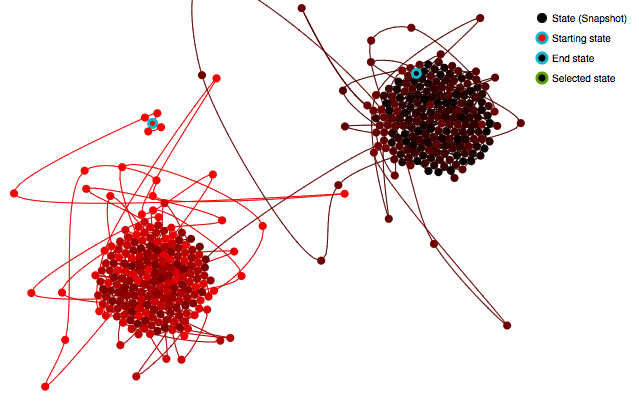
\includegraphics[width=\linewidth]{fig/put-get-curve}%
    \caption{Time curve generated from an etcd raft cluster processing 50 put requests, followed by 50 get requests.\label{fig:put-get-curve}}%
\end{figure}
    


\subsection{Invariant Graph}
\label{sec:invariant-graph}

The invariant graph is composed of points, corresponding to variables,
and edges, which are invariant relationships between the variables.
The invariants Pangaea renders are calculated by Dinv~\cite{dinv}.
Dinv reports invariants in the same format as Daikon~\cite{Ernst01}.
Figure~\ref{fig:dinv-output} is Dinv's invariant output from analyzing
etcd raft. These invariants can be difficult to comprehend for
developers unfamiliar with the format. Further the textual representation
obfuscates the transitive properties of the invariants, requiring the
user to reason about them.

Pangaea graphs the systems invariants to present them intuitively, in a
way which communicates the transitive nature of the invariants. We
implemented four invariant encodings for relationships which hold over
integers, and a subset of which hold over more general types.
Specifically a thin black line denotes equality, while a dashed black
line denotes inequality. Both of these relationships are valid on
arbitrary data so they are graphed for all types, such as strings,
booleans, and integers. Light blue triangular edges correspond to the
\emph{less than} relationship. Two corners of the triangle are attached
to the greater variable, while a single is attached to the lesser.
Similarly a light blue triangle with a black border represents the
\emph{greater than or equal too} relation. Users can select a
variable, and all transitive relations are highlighted in red. When a
variable is highlighted, and variables which do not have a transitive
relationship have their names removed from the graph, to increase
legibility.

Figure~\ref{fig:invariant-graph} is an invariant graph generated from
Dinv's invariant output in Figure~\ref{fig:dinv-output}.
Figure~\ref{fig:invariant-graph}A is the static representation of the
graph.  All variable names, and relationships are visible to the
user. Figure~\ref{fig:invariant-graph}B is the result of a user clicking
on the \emph{C-state} point.

\begin{figure}[h]
    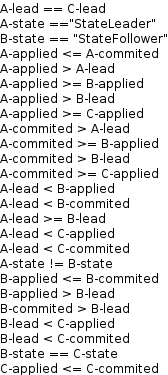
\includegraphics[width=0.5\linewidth]{fig/dinv-output}%
    \caption{Dinv's invariant output from analyzing etcd.\label{fig:dinv-output}}%
\end{figure}

\begin{figure}[h]
    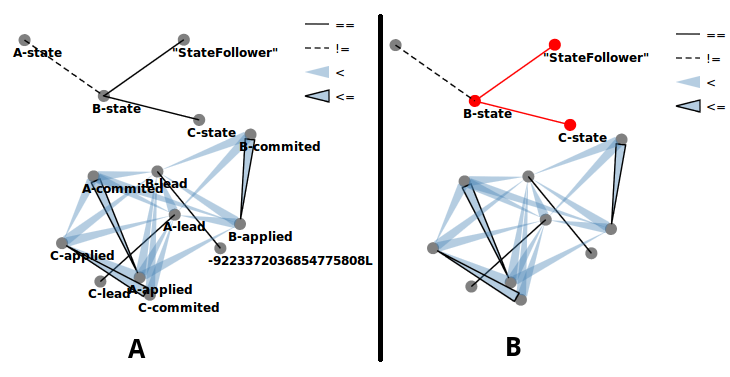
\includegraphics[width=\linewidth]{fig/invariant-graph}%
    \caption{Pangaea's invariant graph generated from Dinv's invariants in Figure~\ref{fig:dinv-output}.A) is a static rendering of the invariants. B) User selected invariants \label{fig:invariant-graph}}%
\end{figure}

\subsection{Communication Graph}
\label{sec:communication-graph}

The communication graph is a directed acyclic graph of node
communication. Vertical lines are unique to individual nodes, and are
assigned a unique color for legibility. At the top of each vertical
line is a square, denote the beginning of an execution, and the name
of the node which the line corresponds to. Circles on each nodes line
are logged events. A diagonal line between events on separate nodes is
a message sent from the node at the top of the diagonal, to the node
at the bottom of the diagonal. Pangaea communication graph is a
re-implementation of ShiViz's visualization~\cite{BeschastnikhWBE2016}.
The purpose of this visual is to help users reason the state of
snapshots. When a user selects a snapshot from the time curve graph
(Section~\ref{sec:time-curve}) gray boxes are added to each node line
at the logical time that the snapshot was taken. This feature allows
users to reason about how specific communication patterns have
influenced the state of their system.

Figure~\ref{fig:communication-graph} is the communication graph of an
etcd raft cluster. The sample is taken from the beginning of an
execution while an initial election takes place, and the nodes of the
cluster agree upon a configuration. The gray boxes correspond to the
logical time of the first snapshot of the system. This visual was
triggered after selecting the initial state from
Figure~\ref{fig:put-get-curve}.


\begin{figure}[h]
    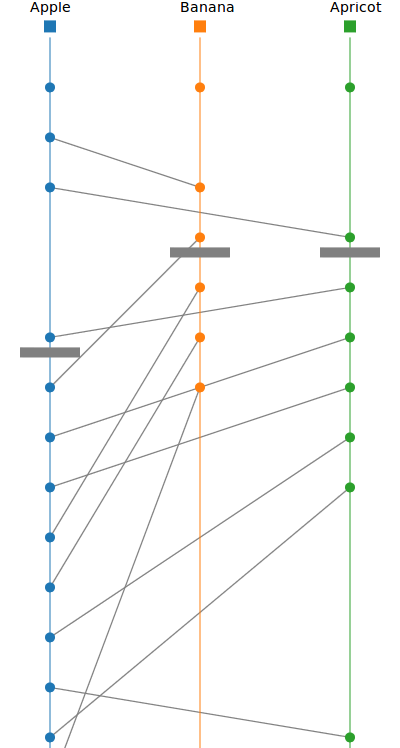
\includegraphics[width=\linewidth]{fig/communication-graph}%
    \caption{Communication graph of an etcd raft election; The first snapshot of the system was selected from the corresponding time curve.\label{fig:communication-graph}}%
\end{figure}



\section{Evaluation}
\label{sec:evaluation}

To evaluate \dviz we will conduct a user study in which participants will use
\dviz to identify buggy distributed systems. The purpose of the study will be
to demonstrate that \dviz's output is useful for detecting buggy executions.
Participants will be shown multiple visualization generated from the executions
of three systems. To demonstrate \dviz's generality the system will be composed
of a cross section of popular distributed applications. Specifically the
systems will be etcd Raft~\cite{etcdraft}, Groupcache~\cite{groupcache} and
Hashicorp Swim~\cite{das2002swim}.  In all cases bugs will be introduced into the
systems and the buggy visualization will be displayed alongside the non-faulty
executions. Etcd Raft will be modified so that leader elections will result in
more than one leader.  Groupcache will not adhere to its key ownership policy.
Swim will not fully propagate event messages to it's cluster. Study participants
will be given a brief description of the systems and will be asked to select the
visualization which they suspect to be faulty. Upon selecting a visualization
participants will be asked to identify which aspects of the visual prompted
their choice.  Finally, they will be shown snippets of source code from the
buggy execution, and be asked to identify the block of code responsible for the
irregular visualization.





\balance
\bibliographystyle{abbrv}
\bibliography{paper}

\end{document}
